
% Mikes: ok
% Spellcheck: ok

% ============================================================
\chapter{More Than Two Variables: Graphical Multivariate Analysis}{}{}
\label{ch:multivariate}

\index{data analysis!multivariate analysis|(} 
\index{multivariate analysis|(} 

\Fint{As soon as we are dealing with more than two variables
simultaneously, things become much more} complicated---in particular,
graphical methods quickly become impractical. In this chapter, I'll
introduce a number of graphical methods that can be applied to
multivariate problems. All of them work best if the number of variables
is not \emph{too} large (less than 15--25).

The borderline case of \emph{three} variables can be handled through
\emph{false-color plots}, which we will discuss first.

If the number of variables is greater (but not much greater) than
three, then we can construct multiplots from a collection of
individual bivariate plots by scanning through the various parameters
in a systematic way. This gives rise to scatter-plot matrices and
co-plots.

Depicting how an overall entity is composed out of its constituent
parts can be a rather nasty problem, especially if the composition
changes over time. Because this task is so common, I'll treat it
separately in its own section.

Multi-dimensional visualization continues to be a research topic, and in
the last sections of the chapter, we look at some of the more recent
ideas in this field.

One recurring theme in this chapter is the need for adequate tools:
most multi-\break dimensional visualization techniques are either not
practical with paper and pencil, or are outright impossible without a
computer (in particular when it comes to animated techniques).
Moreover, as the number of variables increases, so does the need to
look at a data set from different angles; this leads to the idea of
using interactive graphics for exploration. In the last section, we
look at some ideas in this area.

% ============================================================
\section{False-Color Plots}

\index{multivariate analysis!false-color plots|(} 
\index{false-color plots|(}
\index{color, false-color plots|(}

There are different ways to display information in three variables
(typically, two independent variables and one dependent variable).
Keep in mind that simple is sometimes best! Figure \ref{fig:landau}
shows the function $f(x,a) = x^4/2 + a x^2 - x/2 + a/4$ for various
values of the parameter $a$ in a simple, two-dimensional $xy$ plot.
The shape of the function and the way it changes with $a$ are
perfectly clear in this graph. It is very difficult to display this
function in any other way with comparable clarity.

\begin{figure}
   \centerline{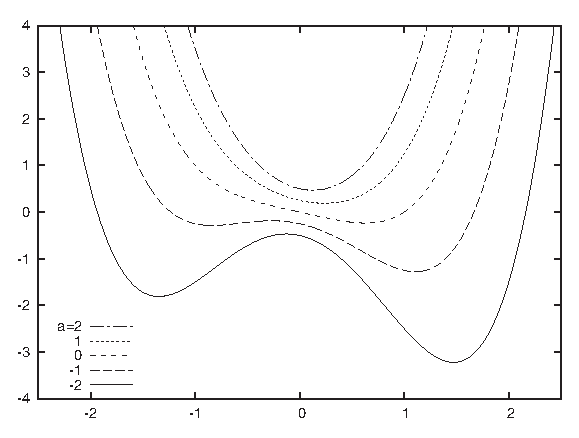
\includegraphics{img/landau}}
  \caption{A simple but effective way to show three variables: treat 
    one as parameter and draw a separate curve for several parameter
    values.}
  \label{fig:landau}\vspace*{12pt}
\end{figure}

Another way to represent such trivariate data is in the form of a
\emph{surface plot}, \index{surface plots} such as the one shown in Figure
\ref{fig:surface}.  As a rule, surface plots are visually stunning but
are of very limited practical utility. Unless the data set is very
smooth and allows for a viewpoint such that we can look \emph{down}
onto the surface, they simply don't work! For example, it is pretty
much impossible to develop a good sense for the behavior of the
function plotted in Figure \ref{fig:landau} from a surface plot. (Try
it!)  Surface plots can help build intuition for the overall
structure of the data, but it is notoriously difficult to read off
quantitative information from them.

\begin{figure}
    \centerline{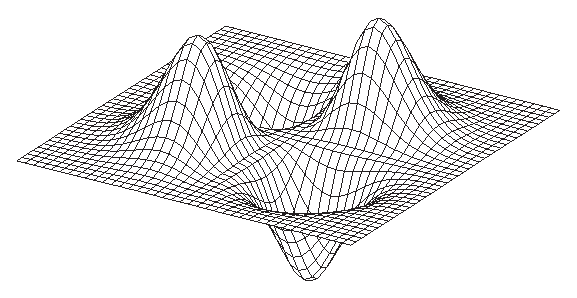
\includegraphics{img/surface}}
  \caption{Surface plots are often visually impressive but generally
    don't represent quantitative information very well.}
  \label{fig:surface}
\end{figure}

In my opinion, surface plots have only two uses:
\begin{enumerate}
\item To get an intuitive impression of the ``lay of the land'' for
  a complicated data set
\item To dazzle the boss (not that this isn't important at times)\vfill\pagebreak
\end{enumerate}

Another approach is to project the function into the base plane below
the surface in Figure \ref{fig:surface}. There are two ways in which
we can represent values: either by showing contours of constant
alleviation in a \emph{contour plot} \index{contour plots} or by mapping the numerical
values to a palette of colors in a \emph{false-color plot}. Contour
plots are familiar from topographic maps---they can work quite well,
in particular if the data is relatively smooth and if one is primarily
interested in local properties.

The false-color plot is an alternative and quite versatile technique
that can be used for different tasks and on a wide variety of data
sets. To create a false-color plot, all values of the dependent
variable $z$ are mapped to a palette of colors. Each data point is
then plotted as a region of the appropriate color. Figure
\ref{fig:grayscale} gives an example (where the color has been
replaced by grayscale shading).

\begin{figure}
   \centerline{\includegraphics{img/falsecolor}}
  \caption{Grayscale version of a false-color plot of the function
    shown as a surface plot in Figure \ref{fig:surface}.  Here white
    corresponds to positive values of the function, and black
    corresponds to negative values.}
  \label{fig:grayscale}
\end{figure}\pagebreak

I like false-color plots because one can represent a lot of
information in a them in a way that retains quantitative information.
However, false-color plots depend crucially on the quality of the
palette---that is, the mapping that has been used to associate colors
with numeric values.

Let's quickly recap some information on color and computer graphics.
Colors for computer graphics are usually specified by a triple of
numbers that specify the intensity of their red, green, and blue (RGB)
components. Although RGB triples make good sense technically, they are
not particularly intuitive. Instead, we tend to think of color in
terms of its hue, saturation, and value (\ie, luminance  or lightness).
Conventionally, hue runs through all the colors of the rainbow (from
red to yellow, green, blue, and magenta). Curiously, the spectrum of
hues seems to circle back onto itself, since magenta smoothly transforms
back to red. (The reason for this behavior is that the hues in the
rainbow spectrum are arranged in order of their dominant
electromagnetic frequency. For violet/magenta, no frequency dominates;
instead, violet is a mixture of low-frequency reds and high-frequency
blues.) Most computer graphics programs will be able to generate color
graphics using a hue--saturation--value (HSV) triple.

It is surprisingly hard to find reliable recommendations on good
palette design, which is even more unfortunate given that convenience
and what seems like common sense often lead to particularly \emph{bad}
palettes. Here are some ideas and suggestions that you may wish to
consider:
\begin{unnumlist}
\subparagraph{Keep it simple}
\item Very simple palettes using red, white, and blue
  often work surprisingly well. For continuous color changes you could
  use a blue-white-red palette, for segmentation tasks you could use
  a white-blue-red-white palette with a sharp blue--red transition
  at the segmentation threshold.

\subparagraph{Distinguish between segmentation tasks and the display of smooth
  changes}
\item Segmentation tasks (\eg, finding all points that exceed a
  certain threshold, finding the locations where the data crosses
  zero) call for palettes with sharp color transitions at the
  respective thresholds, whereas representing smooth changes in a data
  set calls for continuous color gradients. Of course, both aspects
  can be combined in a single palette: gradients for part of the
  palette and sharp transitions elsewhere.

\subparagraph{Try to maintain an intuitive sense of ordering}
\item Map low values
  to ``cold'' colors and higher values to ``hot'' colors to provide an
  intuitive sense of ordering in your palette. Examples include the
  simple blue-red palette and the ``heat scale'' 
  (black-red-yellow-white---I'll discuss in a moment why I don't
  recommend the heat scale for use). Other palettes that convey a
  sense of ordering (if only by convention) are the ``improved
  rainbow'' (blue-cyan-green-\break yellow-orange-red-magenta) and the
  ``geo-scale'' familiar from topographic maps
  (blue-cyan-green-brown-tan-white).\pagebreak

\subparagraph{Place strong visual gradients in regions with important changes}
\item
  Suppose that you have a data set with values that span the range
  from $-100$ to $+100$ but that all the really interesting or
  important change occurs in the range $-10$ to $+10$. If you use a
  standard palette (such as the improved rainbow) for such a data set,
  then the actual region of interest will appear to be all of the same
  color, and the rest of the spectrum will be ``wasted'' on parts of
  the data range that are not that interesting.  To avoid this
  outcome, you have to compress the rainbow so that it maps only to
  the region of interest. You might want to consider mapping the
  extreme values (from $-100$ to $-10$ and from $10$ to $100$) to some
  unobtrusive colors (possibly even to a grayscale) and reserving the
  majority of hue changes for the most relevant part of the data
  range.

\subparagraph{Favor subtle changes}
\item This is possibly the most surprising
  recommendation. When creating palettes, there is a natural tendency
  to ``crank it up full'' by using fully saturated colors at maximal
  brightness throughout. That's not necessarily a good idea, because
  the resulting effect can be so harsh that details are easily lost.
  Instead, you might want to consider using soft, pastel colors or
  even to experiment with mixed hues in favor of the pure primaries of
  the standard rainbow. (Recent versions of Microsoft Excel provide an
  interesting and easily accessible demonstration for this idea: all
  default colors offered for shading the background of cells are soft,
  mixed pastels---to good effect.)  Furthermore, the eye is quite
  good at detecting even subtle variations.  In particular, when
  working with luminance-based palettes, small changes are often all
  that is required.

\subparagraph{Avoid changes that are hard to detect}
\item Some visual changes are
  especially hard to perceive visually. For example, it is practically
  impossible to distinguish between different shades of yellow, and
  the transition from yellow to white is even worse!  (This is why I
  don't recommend the heat scale, despite its nice ordering property:
  the bottom third consists of hard-to-distinguish dark reds, and the
  entire upper third consists of very hard-to-distinguish shades of
  light yellow.)

\subparagraph{Use hue- and luminance-based palettes for different purposes}
\item In
  particular, consider using a luminance-based palette to emphasize
  fine detail and using hue- or saturation-based palettes for smooth,
  large-scale changes. There is some empirical evidence that
  luminance-based palettes are better suited for images that contain a
  lot of fine detail and that hue-based palettes are better suited for
  bringing out smooth, global changes. A pretty striking demonstration
  of this observation can be found when looking at medical images
  (surely an application where details matter!): a simple grayscale
  representation, which is pure luminance, often seems much clearer
  than a multicolored representation using a hue-based rainbow
  palette.  This rule is more relevant\vadjust{\pagebreak} to image processing of
  photographs or similar images (such as that in our medical example)
  than to visualization of the sort of abstract information that we
  consider here, but it is worth keeping in mind.
  
\subparagraph{Don't forget to provide a color box}
\item No matter how intuitive you
  think your palette is, nobody will know for sure what you are
  showing unless you provide a color box (or color key) that shows the
  values and the colors they are mapped to.  Always, always, provide
  one.
\end{unnumlist}

One big problem not properly addressed by these recommendations
concerns \emph{visual uniformity}. \index{visual uniformity} For example, consider palettes
based on the ``improved rainbow,'' which is created by distributing
the six primaries in the order blue-cyan-green-yellow-red-magenta
across the palette. If you place these primaries at equal distances
across from each other and interpolate linearly between them in color
space, then the fraction of the palette occupied by green appears to
be much larger than the fraction occupied by either yellow or cyan.
Another example is that when placing a fully saturated yellow next to
a fully saturated blue, then the blue region will appear to be more
intense (\ie, saturated) than the yellow. Similarly, the browns that
occur in a geo-scale easily appear darker than the other colors in the
palette. This is a problem with our \emph{perception} of color: simple
interpolations in color space do not necessarily result in visually
uniform gradients!

There is a variation of the HSV color space, called the \emph{HCL}
(hue--chroma--luminance) space \index{HCL (hue--chroma--luminance) space} that takes visual perception into
account to generate visually uniform color maps and gradients.  The
HCL color model is more complicated to use than the HSV model, because
not all combinations of hue, chroma, and luminance values exist.  For
instance, a fully saturated yellow appears lighter than a fully
saturated blue, so a palette at full chroma and with high luminance
will include the fully saturated yellow but not the blue. As a result,
HCL-based palettes that span the entire rainbow of hues tend naturally
toward soft, pastel colors.  A disadvantage of palettes in the HCL
space is that they often degrade particularly poorly when reproduced
in black and white.\footnote{An implementation of the transformations
  between HCL and RGB is available in R and C in the ``colorspace''
  module available from CRAN.}

A special case of false-color plots are geographic \emph{maps}, and
cartographers have significant experience developing color schemes for
various purposes. Their needs are a little different and not all of
their recommendations may work for general data analysis purposes, but
it is worthwhile to become familiar with what they have
learned.\footnote{An interesting starting point is Cynthia Brewer's
  online ColorBrewer at \url{http://colorbrewer2.org/}.}

Finally, I'd like to point out two additional problems with all
plots that depend on color to convey critical information.

\begin{itemize}
\item Color does not reproduce well. Once photocopied or printed on a
  black-and-white laser printer, a false-color plot will become
  useless!
\item Also keep in mind that about 10 percent of all men are at least
  partially color blind; these individuals won't be able to make much
  sense of most images that rely heavily or exclusively on color.
\end{itemize}

Either one of these problems is potentially serious enough that you
might want to reconsider before relying entirely on color for the
display of information.

In my experience, preparing good false-color plots is often a tedious
and time-consuming task. This is one area where better tools would be
highly desirable---an interactive tool that could be used to
manipulate palettes directly and in real time would be very nice to
have. The same is true for a publicly available set of well-tested
palettes.

\index{multivariate analysis!false-color plots|)} 
\index{false-color plots|)}
\index{color, false-color plots|)}

% ============================================================
\section{A Lot at a Glance: Multiplots}

\index{multivariate analysis!multiplots|(} 
\index{multiplots|(} 

The primary concern in all multivariate visualizations is finding
better ways to put more ``stuff'' on a graph. In addition to color
(see the previous section), there are basically two ways we can go
about this. We can make the graph elements themselves richer, so that
they can convey additional information beyond their position on the
graph; or we can put several similar graphs next to each other and
vary the variables that are not explicitly displayed in a systematic
fashion from one subgraph to the next. The first idea leads to
\emph{glyphs}, which we will introduce later in this chapter, whereas
the latter idea leads to scatter-plot matrices and co-plots.

\subsection{The Scatter-Plot Matrix}

\index{multiplots!scatter-plot matrices|(} 
\index{scatter-plot matrices|(} 

For a \emph{scatter-plot matrix} (occasionally abbreviated SPLOM), we
construct all possible two-dimensional scatter plots from a
multivariate data set and then plot them together in a matrix format
(Figure \ref{fig:splom}). We can now scan all of the graphs for
interesting behavior, such as a marked correlation between any two
variables.

\begin{figure}
  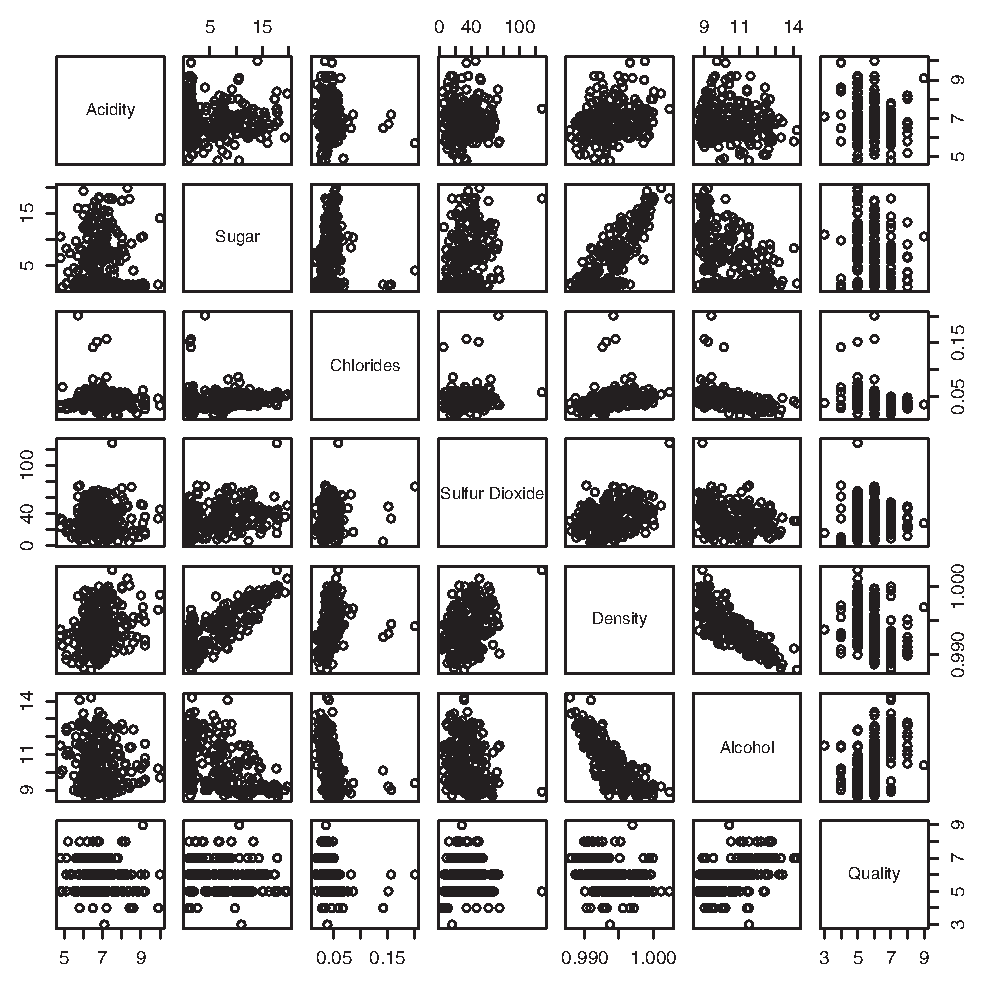
\includegraphics[width=\textwidth]{img/splom.eps}
  \caption{In a scatter-plot matrix (SPLOM), a separate scatter plot is
    shown for each pair of variables. All scatter plots in a given row
    or column have the same plot range, so that we can compare them
    easily.}
  \label{fig:splom}\vspace*{-6pt}
\end{figure}

The data set shown in Figure \ref{fig:splom} consists of seven
different properties of a sample of 250 wines.\footnote{The data can
  be found in the ``Wine Quality'' data set, available at the UCI
  Machine Learning repository at
  \url{http://archive.ics.uci.edu/ml/}.} It is not
at all clear how these properties should relate to each other, but by
studying the scatter-plot matrix, we can make a few interesting
observations. For example, we can see that sugar content and density
are positively correlated: if the sugar content goes up, so does the
density. The opposite is true for alcohol content and density: as the
alcohol content goes up, density goes down. Neither of these
observations should come as a surprise (sugar syrup has a higher
density than water and alcohol a lower one). What may be more interesting
is that the wine quality seems to increase with increasing alcohol
content: apparently, more potent wines are considered to be better!

One important detail that is easy to overlook is that all graphs in
each row or column show the same plot range; in other words, they
use \emph{shared scales}. This makes it possible to compare graphs
across the entire matrix. 

The scatter-plot matrix is symmetric across the diagonal: the subplots
in the lower left are equal to the ones in the upper right but rotated
by 90 degrees. It is nevertheless customary to plot both versions
because this makes it possible to scan a single row or column in its
entirety to investigate how one quantity relates to each of the other
quantities.

Scatter-plot matrices are easy to prepare and easy to understand. This
makes them very popular, but I think they can be overused. Once we
have more than about half a dozen variables, the individual subplots\vadjust{\pagebreak}
become too small as that we could still recognize anything useful, in
particular if the number of points is large (a few hundred points or
more). Nevertheless, scatter-plot matrices are a convenient way to
obtain a quick overview and to find viewpoints (variable pairings)
that deserve a closer look.
\index{multiplots!scatter-plot matrices|)}% 
\index{scatter-plot matrices|)}% 

\subsection{The Co-Plot}

\index{multiplots!coplots|(} 
\index{coplots|(} 

In contrast to scatter-plot matrices, which always show all data
points but \emph{project} them onto different surfaces of the
parameter space, \emph{co-plots} (short for ``conditional plots'')
show various \emph{slices} through the parameter space such that each
slice contains only a subset of the data points. The slices are taken
in a systematic manner, and we can form an image of the entire
parameter space by mentally gluing the slices back together again
(the salami principle). Because of the regular layout of the subplots,
this technique is also known as a \emph{trellis plot}.

Figure \ref{fig:coplot1} shows a trivariate data set projected onto
the two-dimensional $xy$ plane. Although there is clearly structure in
the data, no definite pattern emerges. In particular, the dependence
on the third parameter is entirely obscured!

Figure \ref{fig:coplot2} shows a co-plot of the same data set that is
sliced or \emph{conditioned} on the third parameter $a$.  The bottom 
part of the graph shows six slices through the data corresponding to
different ranges of $a$. (The slice for the \emph{smallest} values of
$a$ is in the lower left, and the one for the largest values of $a$
is in the upper righthand corner.) As we look at the slices, the
structure in the data stands out clearly, and we can easily follow the
dependence on the third parameter $a$.

The top part of Figure \ref{fig:coplot2} shows the range of values
that $a$ takes on for each of the slices. If you look closely, you
will find that there are some subtle issues hidden in (or rather
revealed by) this panel, because it provides information on the
details of the slicing operation.

\begin{figure}[t!]
   \centerline{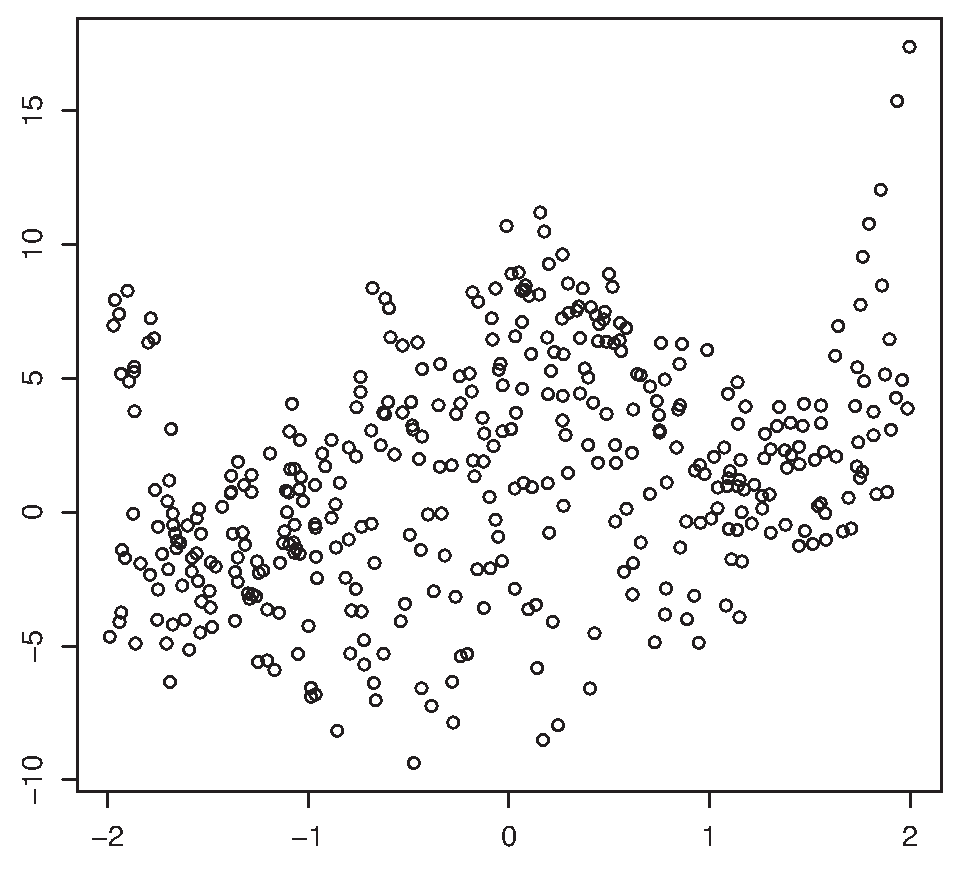
\includegraphics[width=0.8\textwidth]{img/coplot1.eps}}
  \caption{Projection of a trivariate data set onto the $xy$ plane. 
    How does the data vary with the third variable?}
  \label{fig:coplot1}
\end{figure}

Two decisions need to be made with regard to the slicing:
\begin{enumerate}
\item By what method should the overall parameter range be cut into
  slices?
\item Should slices overlap or not?
\end{enumerate}

In many ways, the most ``natural'' answer to these questions would be
to cut the entire parameter range into a set of adjacent intervals of
equal width. It is interesting to observe (by looking at the top panel
in Figure \ref{fig:coplot2}) that in the example graph, a different
decision was made in regard to both questions! The slices are 
not of equal width in the range of parameter values that they span;
instead, they have been made in such a way that each slice contains
\emph{the same number of points}. Furthermore, the slices are not
adjacent but partially overlap each other.

The first decision (to have each slice contain the same number of
points, instead of spanning the same range of values) is particularly
interesting because it provides additional\vadjust{\pagebreak} information on how the
values of the parameter $a$ are distributed. For instance, we can see
that large values of $a$ (larger than about $a=-1$) are relatively
rare, whereas values of $a$ between $-4$ and $-2$ are much more
frequent. This kind of behavior would be much harder to recognize
precisely if we had chopped the interval for $a$ into six slices of
equal width. The other decision (to make the slices overlap partially)
is more important for small data sets, where otherwise each slice
contains so few points that the structure becomes hard to see.  Having
the slices overlap makes the data ``go farther'' than if the slices
were entirely disjunct.

Co-plots are especially useful if some of the variables in a data set
are clearly ``control'' variables, because co-plots provide a
systematic way to study the dependence of the remaining (``response'')
variables on the controls.
\index{multiplots!coplots|)} 
\index{coplots|)} 


\begin{figure}
  \centerline{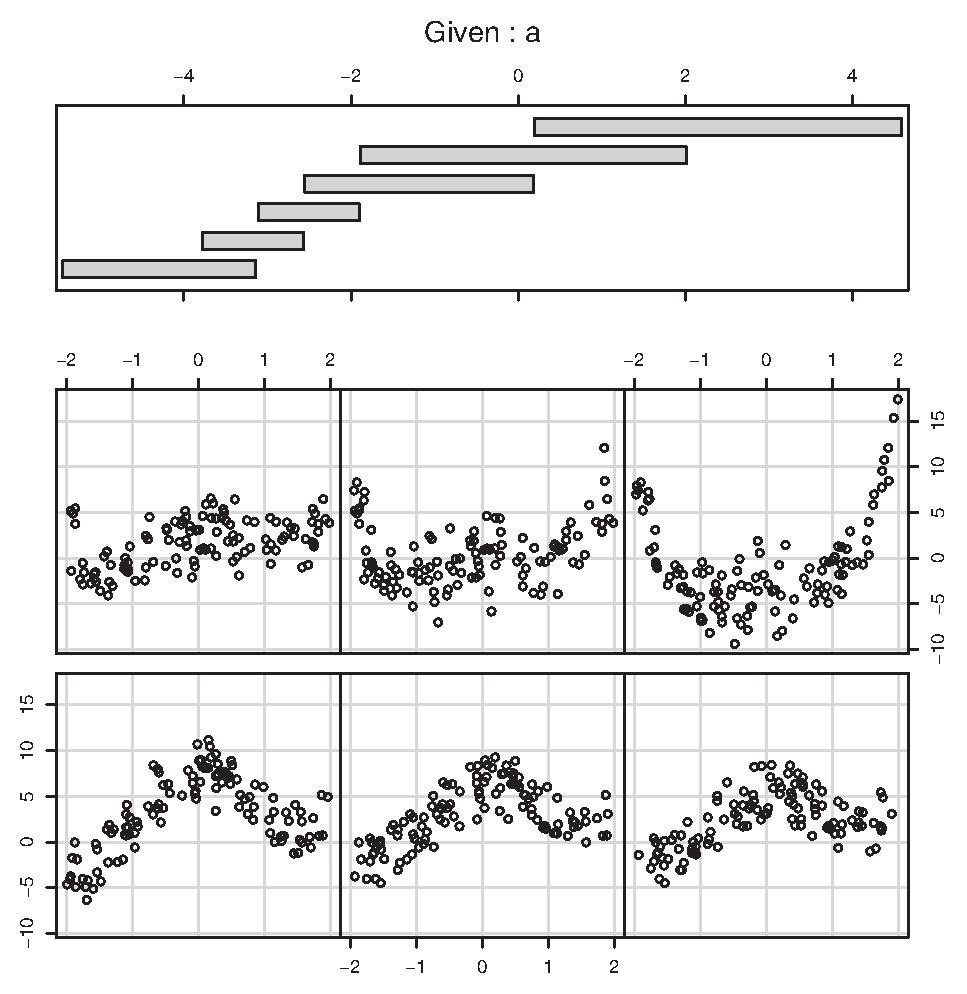
\includegraphics[width=0.8\textwidth]{img/coplot2.eps}}
  \caption{A co-plot of the same data as in Figure \ref{fig:coplot1}.
    Each scatter plot includes the data points for only a certain
    range of $a$ values; the corresponding values of $a$ are shown in
    the top panel.  (The scatter plot for the smallest value of $a$ is
    in the lower left corner, and that for the largest value of $a$ is
    in the upper right.)}
  \label{fig:coplot2}\vspace*{-6pt}
\end{figure}

\vspace*{-6pt}
\subsection{Variations}

The ideas behind scatter-plot matrices and co-plots are pretty 
generally applicable, and you can develop different variants
depending on your needs and tastes. Here are some ideas:

\begin{itemize}
\item In the standard scatter-plot matrix, half of the individual
  graphs are redundant. You can remove the individual graphs from half
  of the overall matrix and replace them with something
  different---for example, the numerical\vadjust{\pagebreak} value of the appropriate
  correlation coefficient.  However, you will then lose the ability to
  visually scan a full row or column to see how the corresponding
  quantity correlates with all other variables.
\item Similarly, you can place a histogram showing the distribution
  of values for the quantity in question on the diagonal of the 
  scatter-plot matrix.\index{histograms!scatter-plot matrices}
\item The slicing technique used in co-plots can be used with other
  graphs besides scatter plots. For instance, you might want to use
  slicing with rank-order plots (see Chapter \ref{ch:univariate}),
  where the conditioning ``parameter'' is some quantity not explicitly
  shown in the rank-order plot itself. Another option is to use it
  with histograms, making each subplot a histogram of a subset of the
  data where the subset is determined by the values of the control
  ``parameter'' variable.
\item Finally, co-plots can be extended to \emph{two} conditioning
  variables, leading to a matrix of individual slices.
\end{itemize}

By their very nature, all multiplots consist of many individual plot
elements, sometimes with nontrivial interactions (such as\vadjust{\pagebreak} the
overlapped slicing in certain co-plots). Without a good tool that
handles most of these issues automatically, these plot types lose
most of their appeal. For the plots in this section, I used R (the
statistical package), which provides support for both scatter-plot
matrices and co-plots as built-in functionality.

\index{multivariate analysis!multiplots|)} 
\index{multiplots|)} 

\vspace*{-6pt}
% ============================================================
\section{Composition Problems}

\index{multivariate analysis!composition problems|(} 
\index{composition, multivariate analysis|(} 

Many data sets describe a \emph{composition problem}; in other words,
they describe how some overall quantity is composed out of its parts.
Composition problems pose some special challenges because often we
want to visualize two \emph{different} aspects of the data
simultaneously: on the one hand, we are interested in the relative
magnitude of the different components, and on the other,  we also care
about their absolute size.

For one-dimensional problems, this is not too difficult (see Chapter
\ref{ch:univariate}). We can use a histogram or a similar graph to
display the absolute size for all components; and we can use a
cumulative distribution plot (or even the much-maligned pie chart) to
visualize the relative contribution that each component makes to the
total.

But once we add additional variables into the mix, things can get
ugly. Two problems stand out: how to visualize \emph{changes} to the
composition over time and how to depict the breakdown of an overall
quantity along \emph{multiple axes} at the same time.

\vspace*{-6pt}
\subsection{Changes in Composition}

To understand the difficulties in tracking compositional problems over
time, imagine a company that makes five products labeled A, B, C, D,
and E. As we track the daily production numbers over time, there are
two different questions that we are likely to be interested in: on the
one hand, we'd like to know how many items are produced overall; on
the other hand, we would like to understand how the item mix is
changing over time.

\begin{figure}
  \centerline{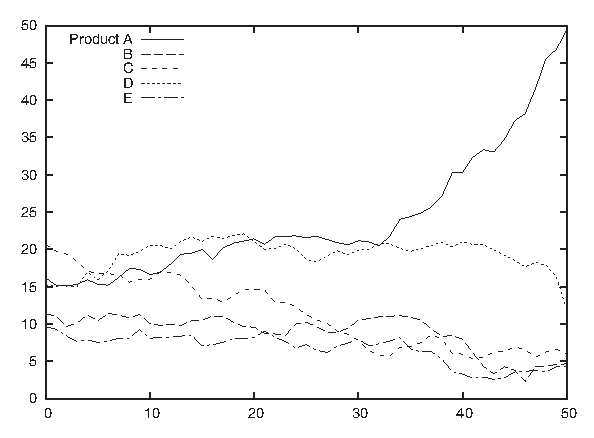
\includegraphics{img/composition1}}
  \caption{Absolute number of items produced per product line and day.}
  \label{fig:composition1}
\end{figure}

Figures \ref{fig:composition1}, \ref{fig:composition2}, and
\ref{fig:composition3} show three attempts to plot this kind of data.
Figure \ref{fig:composition1} simply shows the absolute numbers
produced per day for each of the five product lines. That's not
ideal---the graph looks messy because some of the lines obscure each
other.  Moreover, it is not possible to understand from this graph how
the total number of items changes over time. Test yourself: does the
total number of items go up over time, does it go down, or does it
stay about even?

Figure \ref{fig:composition2} is a \emph{stacked plot} \index{stacked plots} of the same
data. The daily numbers for each product are added to the numbers for
the products that appear lower down in the diagram---in other words,
the line labeled B gives the number of items produced in product lines
A \emph{and} B. The topmost line in this diagram shows the total
number of items produced per day (and answers the question posed in
the previous paragraph: the total number of items does \emph{not}
change appreciably over the long run---a possibly surprising
observation, given the appearance of Figure \ref{fig:composition1}).

\begin{figure}
  \centerline{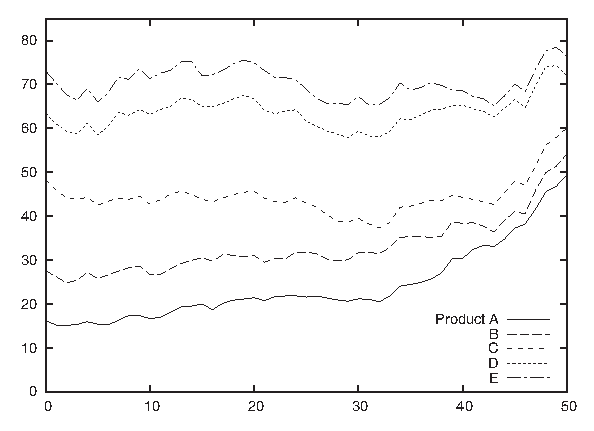
\includegraphics{img/composition2}}
  \caption{Stacked graph of the number of items produced per product
    line and day.}
  \label{fig:composition2}
\end{figure}

Stacked plots can be compelling because they have intuitive appeal and
appear to be clear and uncluttered. In reality, however,\vadjust{\pagebreak} they tend to
hide the details in the development of the individual components
because the changing baseline makes comparison difficult if not
impossible.  For example, from Figure \ref{fig:composition1} it is
pretty clear that production of item D increased for a while but then
dropped rapidly over the last 5 to 10 days. We would never guess this
fact from Figure \ref{fig:composition2}, where the strong growth of
product line A masks the smaller changes in the other product lines.
(This is why you should order the components in a stacked graph in
ascending order of variation---which was intentionally \emph{not} done
in Figure \ref{fig:composition2}.)

Figure \ref{fig:composition3} shows still another attempt to visualize
this data. This figure is also a stacked graph, but now we are looking
not at the absolute numbers of items produced but instead at the
relative fraction that each product line contributes to the daily
total. Because the change in the total number of items produced has
been eliminated, this graph can help us understand how the item mix
varies over time (although we still have the changing baseline problem
common to all stacked graphs). However, information about the total
number of items produced has been lost.

\begin{figure}
  \centerline{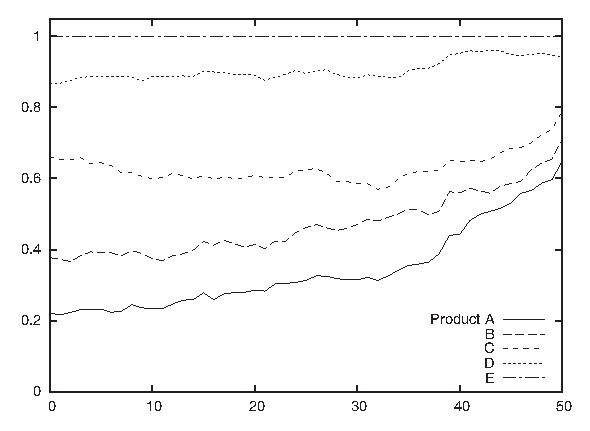
\includegraphics{img/composition3}}
  \caption{Stacked graph of the relative contribution that each
    product line makes to the total.}
  \label{fig:composition3}\vspace*{-6pt}
\end{figure}

All things considered, I don't think any one of these graphs succeeds
very well. No single graph can satisfy both of our conflicting
goals---to monitor both absolute numbers as well as relative
contributions---and be clear and visually attractive at the same time.

I think an acceptable solution for this sort of problem will always
involve a combination of graphs---for example, one for the total
number of items produced and another for the relative item mix.
Furthermore, despite their aesthetic appeal, stacked graphs should be
avoided because they make it too difficult to recognize relevant
information in the graph. A plot such as Figure \ref{fig:composition1}
may seem messy, but at least it can be read accurately and reliably.

\subsection{Multidimensional Composition: Tree and Mosaic Plots}

\index{tree plots, multidimensional composition|(} 
\index{mosaic plots, multidimensional composition|(} 

Composition problems are generally difficult even when we do not worry
about changes over time. Look at the following data:

\begin{verbatim}
Male    BS      NYC     Engineering
Male    MS      SFO     Engineering
Male    PhD     NYC     Engineering
\end{verbatim}
\begin{verbatim}
Male    BS      LAX     Engineering
Male    MS      NYC     Finance
Male    PhD     SFO     Finance
Female  PhD     NYC     Engineering
Female  MS      LAX     Finance
Female  BS      NYC     Finance
Female  PhD     SFO     Finance
\end{verbatim}

The data set shows information about ten employees of some company,
and for each employee, we have four pieces of information: gender,
highest degree obtained, office where they are located (given by
airport code---NYC: New York, SFO: San Francisco, LAX: Los Angeles),
and their department. Keep in mind that each line corresponds to a
single person.

The usual way to summarize such data is in the form of a \emph{contingency
  table}. \index{contingency tables} Table \ref{tbl:mosaicplot} summarizes what we know about the
relationship between an employee's gender and his or her department.
Contingency tables are used to determine whether there is a correlation
between categorical variables: in this case, we notice that men tend
to work in engineering and women in finance. (We may want to divide
by the total number of records to get the \emph{fraction} of employees
in each cell of the table.)

\begin{table}[b]
\def\a{\hphantom{0}}
\def\vrl{\smash{\vrule height48.6pt  width.25pt depth5pt}}
\tbl{A contingency table: breakdown of male and female employees
  across two departments\label{tbl:mosaicplot}}{%
\begin{tabular}{l@{\hskip9pt}c@{\hskip9pt}cc@{\hskip9pt}c@{\hskip9pt}c}\toprule
                               && \TCH{Male} & \TCH{Female} && \TCH{Total} \\\colrule
Engineering     && 4    & 1      && \a5  \\
Finance         && 2    & 3      && \a5 \\\colrule
\textbf{Total}  &\vrl& 6    & 4      &\vrl& 10\\\botrule
\end{tabular}}
\end{table}

The problem is that contingency tables only work for two dimensions at
a time. If we also want to include the breakdown by degree or
location, we have no other choice than to repeat the basic structure
from Table \ref{tbl:mosaicplot} several times: once for each office or
once for each degree.

A \emph{mosaic plot} is an attempt to find a graphical representation
for this kind of data. The construction of a mosaic plot is
essentially recursive and proceeds as follows (see Figure
\ref{fig:mosaicplots}):

\begin{enumerate}
\item Start with a square.
\item Select a dimension, and then divide the square proportionally
  according to the counts for this dimension.
\item Pick a second dimension, and then divide each subarea according
  to the counts along the second dimension, separately for each
  subarea.
\item Repeat for all dimensions, interchanging horizontal and vertical
  subdivisions for each new dimension.
\end{enumerate}

In the lower left panel of Figure \ref{fig:mosaicplots}, location is shown as a secondary vertical subdivision in 
addition to the gender (from left to right: LAX, NYC, SFO). In
addition, the degree is shown through shading (shaded sections
correspond to employees with a Ph.D.).

\begin{figure}
  \begin{tabular}{@{\hskip-12pt}cc}
    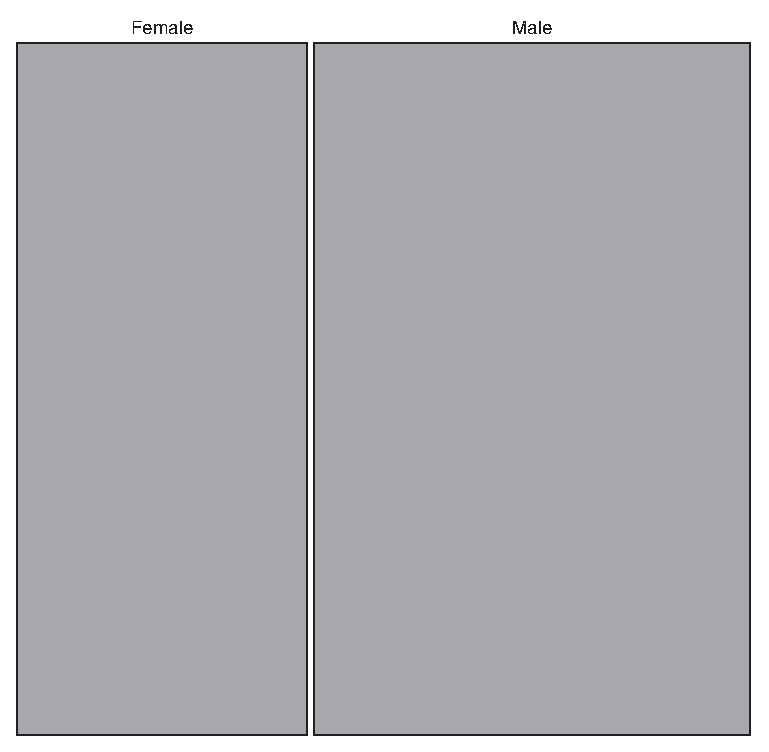
\includegraphics[width=2.5in]{img/mosaic1} &
    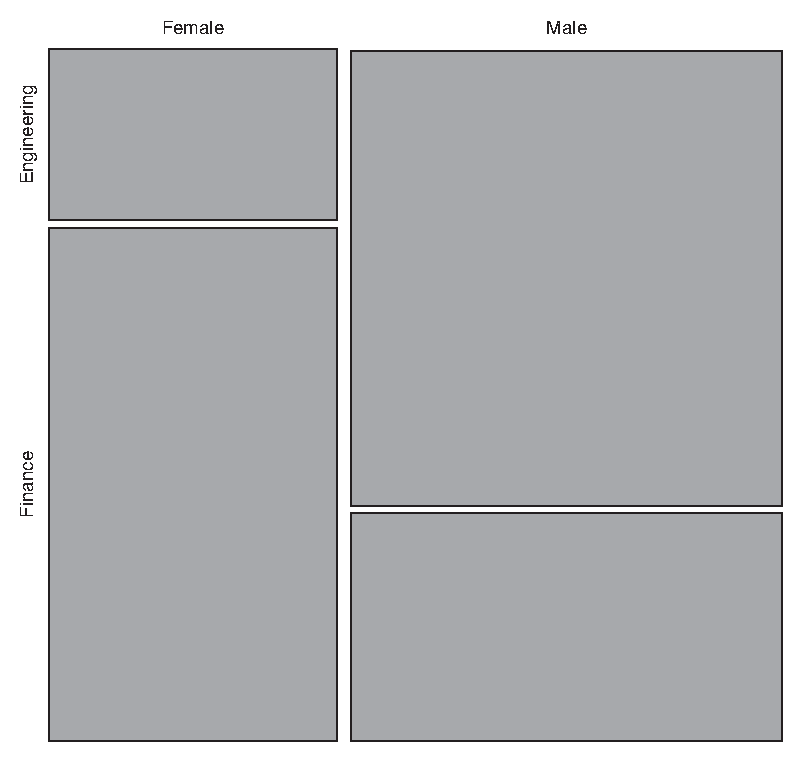
\includegraphics[width=2.5in]{img/mosaic2} \\[6pt]
    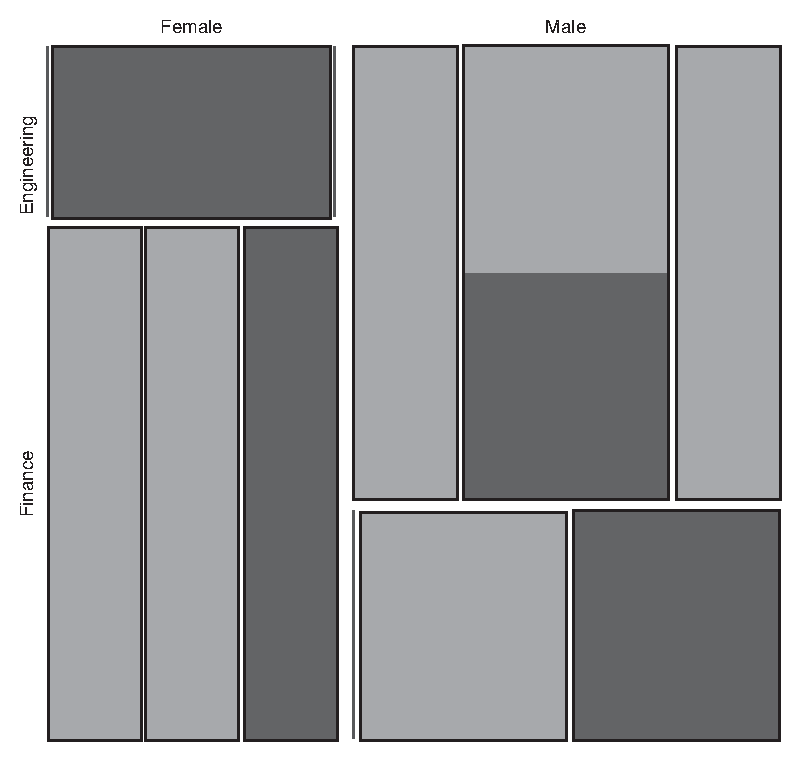
\includegraphics[width=2.5in]{img/mosaic3} &
    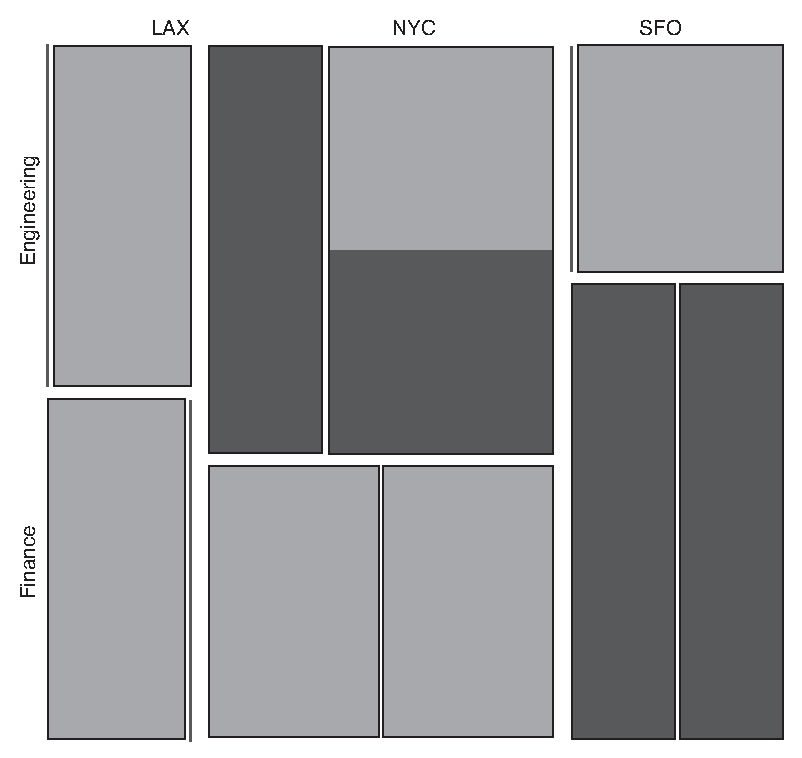
\includegraphics[width=2.5in]{img/mosaic4} 
  \end{tabular}
  \caption{Mosaic plots. In the top row, we start by dividing by 
    gender, then also by department. In the bottom row, we have
    divided by gender, department, and location, with doctorate
    degrees shaded. The graph on the left uses the same sort order
    of dimensions as the graphs in the top row, whereas the graph
    on the bottom right uses a different sort order. Notice how
    the sort order changes the appearance of the graph!}
  \label{fig:mosaicplots}
\end{figure}

Having seen this, we should ask how much mosaic plots actually help us
understand this data set.  Obviously, Figure \ref{fig:mosaicplots} is
difficult to read and has to be studied carefully. Keep in mind that
the information about the number of data points within each category
is represented by the area---recursively at all levels. Also note that
some categories are empty and therefore invisible (for instance, there
are no female employees in either the Los Angeles or San Francisco
engineering departments).

I appreciate mosaic plots because they represent a new idea for how
data can be displayed graphically, but I have not found them to be
useful.  In my own experience, it is easier to understand a data set
by poring over a set of contingency tables than by drawing mosaic
plots.  Several problems stand out.

\begin{itemize}
\item The order in which the dimensions are applied matters greatly
  for the appearance of the plot. The lower right panel in Figure
  \ref{fig:mosaicplots} shows the same data set yet again, but this
  time the data was split along the location dimension first and
  along the gender dimension last.  Shading again indicates employees
  with a Ph.D. Is it obvious that this is the same data set? Is one
  representation more helpful than the other?
\item Changing the sort order changes more than just the appearance, it
  also influences what we are likely to recognize in the graph. Yet
  even with an interactive tool, I find it thoroughly confusing to
  view a large number of mosaic plots with changing layouts. 
\item It seems that once we have more than about four or five
  dimensions, mosaic plots become too cluttered to be useful. This is
  not a huge advance over the two dimensions presented in basic
  contingency tables!
\item Finally, there is a problem common to all visualization methods
  that rely on \emph{area} to indicate magnitude: human perception is
  not that good at comparing areas, especially areas of different
  shape. In the lower right panel in Figure \ref{fig:mosaicplots}, for
  example, it is not obvious that the sizes of the two shaded areas
  for engineering in NYC are the same. (Human perception works by
  comparing visual objects to each other, and the easiest to compare
  are lengths, not areas or angles. This is also why you should favor
  histograms over pie charts!)
\end{itemize}

In passing, let's quickly consider a different but related concept:
\emph{tree maps}. Tree maps are area-based representations of
hierarchical tree structures.  As shown in Figure \ref{fig:treemaps},
the area of each parent node in the tree is divided according to the
weight of its children.

\begin{figure}
  \begin{tabular}{ccc}
    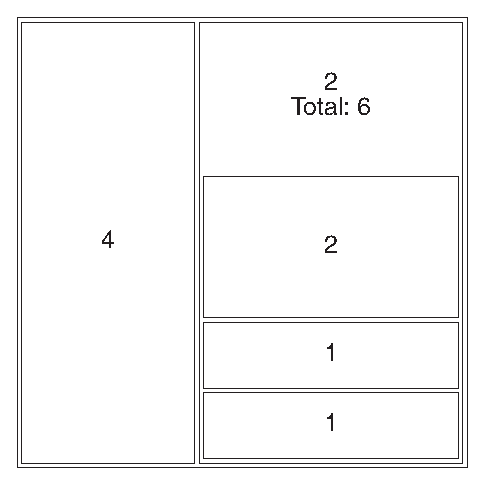
\includegraphics[width=2in]{img/treemap1} &
    \hspace{1cm}
    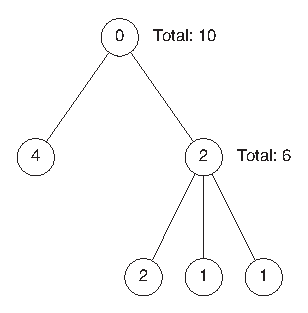
\includegraphics{img/treemap2} 
  \end{tabular}
  \caption{A tree map (left) and the corresponding tree (right). The
    numbers give the weight of each node and, if applicable, also the
    weight of the entire subtree.}
  \label{fig:treemaps}
\end{figure}\pagebreak

Tree maps are something of a media phenomenon.  Originally developed
for the purpose of finding large files in a directory hierarchy, they
seem to be more talked about then used. They share the problems of all
area-based visualizations already discussed, and even their inventors
report that people find them hard to read---especially if the number
of levels in the hierarchy increases. Tree maps lend themselves well
to interactive explorations (where you can ``zoom in'' to deeper
levels of the hierarchy).

My greatest concern is that tree maps have abandoned the primary
advantage of graphical methods without gaining sufficiently in power,
namely \emph{intuition}: looking at a tree map does not conjure up the
image of, well, a \emph{tree}! (I also think that the focus on
treelike hierarchies is driven more by the interests of computer
science, rather than by the needs of data analysis---no wonder if the
archetypical application consisted of browsing a file system!)

\index{tree plots, multidimensional composition|)} 
\index{mosaic plots, multidimensional composition|)} 
\index{multivariate analysis!composition problems|)} 
\index{composition, multivariate analysis|)} 

% ============================================================
\section{Novel Plot Types}

Most of the graph types I have described so far (with the exception of
mosaic plots) can be described as ``classical'': they have been around
for years. In this section, we will discuss a few techniques that are
much more recent---or, at least, that have only recently received
greater attention.

\subsection{Glyphs}

\index{multivariate analysis!glyphs|(} 
\index{glyphs}
 
We can include additional information in any simple plot (such as a
scatter plot) if we replace the simple symbols used for individual
data points with \emph{glyphs}: more complicated symbols that can
express additional bits of information by themselves.

An almost trivial application of this idea occurs if we put two data
sets on a single scatter plot and use different symbols (such as
squares and crosses) to mark the data points from each data set.  Here
the symbols themselves carry meaning but only a simple, categorical
one---namely, whether the point belongs to the first or second data
set.

But if we make the symbols more complicated, then they can express
more information.  Textual labels (letters and digits) are often
surprisingly effective when it comes to conveying more
information---although distinctly low-tech, this is a technique to
keep in mind!

The next step up in sophistication are arrows, which can represent
both a direction and a magnitude (see Figure \ref{fig:vectorplot}), but
we need not stop there. Each symbol can be a fully formed graph (such
as a pie chart or a histogram) all by itself. And even that is not the
end---probably the craziest idea in this realm are ``Chernoff faces,''
where different quantities are encoded as \emph{facial features} (\eg,
size of the mouth, distance between the eyes), and the faces are used
as symbols on a plot!

As you can see, the problem lies not so much in putting more
information on a graph as in being able to interpret the result in a
useful manner. And that seems to depend mostly on the \emph{data}, in
particular on the presence of large-scale, regular structure in it.
If such structure is missing, then plots using glyphs can be very hard
to decode and quite possibly useless.

\begin{figure}
  \centerline{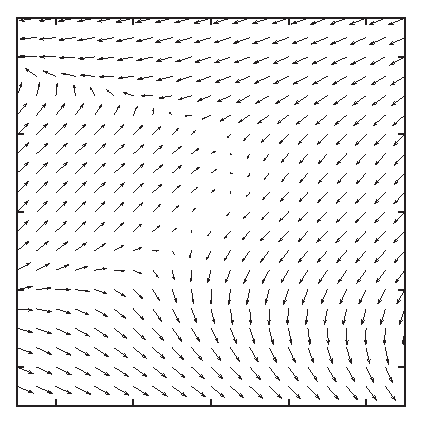
\includegraphics{img/vectorplot}}
  \caption{Simple glyphs: using arrows to indicate both direction and
    magnitude of a field. Notice that the variation in the data is
    smooth and that the data itself has been recorded on a regular
    grid.}
  \label{fig:vectorplot}\vspace*{-6pt}
\end{figure}

Figures \ref{fig:vectorplot} and \ref{fig:glyphplot} show two extreme
examples. In Figure \ref{fig:vectorplot}, we visualize a
four-dimensional data set using arrows (each point of the
two-dimensional plot area has both a direction and a magnitude, so the
total number of dimensions is four). You can think of the system as
flow in a liquid, as electrical or magnetic field lines, or as
deformations in an elastic medium---it does not matter, the overall
nature of the data becomes quite clear. But Figure \ref{fig:glyphplot}
is an entirely different matter! Here we are dealing with a data set
in seven dimensions: the first two are given by the position of the
symbol on the plot, and the remaining five are represented via
distortions of a five-edged polygon.  Although we can make out some
regularities (\eg, the shapes of the symbols in the lower lefthand
corner are all quite similar and different from the shapes elsewhere),
this graph is hard to read and does not reveal the overall
structure of the data very well. Also keep in mind that the
appearance of the graph will change if we map a different pair of
variables to the main axes of the plot, or even if we change the order
of variables in the polygons.

\begin{figure}
   \centerline{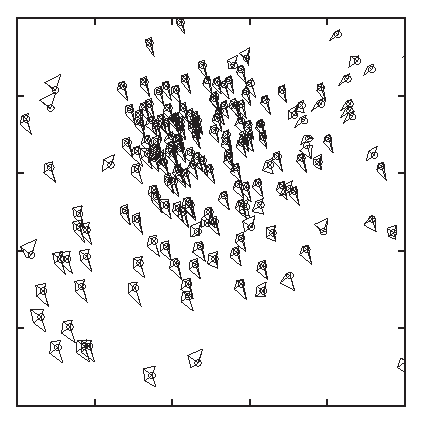
\includegraphics{img/glyphplot}}
  \caption{Complex glyphs: each polygon encodes five different
    variables, and its position on the plot adds another two.}
  \label{fig:glyphplot}
\end{figure}

\vspace*{-6pt}
\subsection{Parallel Coordinate Plots}

\index{multivariate analysis!parallel coordinate plots|(}
\index{parallel coordinate plots|(}  

As we have seen, a scatter plot can show two variables. If we use
glyphs, we can show more, but not\vadjust{\pagebreak} all variables are treated equally
(some are encoded in the glyphs, some are encoded by the position of
the symbol on the plot). By using \emph{parallel coordinate plots}, we
can show all the variables of a multivariate data set on equal footing.
The price we pay is that we end up with a graph that is neither pretty
nor particularly intuitive, but that can be useful for exploratory
work nonetheless.

In a regular scatter plot in two (or even three) dimensions, the
coordinate axes are at right angles to each other. In a parallel
coordinate plot, the coordinate axes instead are \emph{parallel} to
each other. For every data point, its value for each of the variables
is marked on the corresponding axis, and then all these points are
connected with lines. Because the axes are parallel to each other, we
don't run out of spatial dimensions and therefore can have as many
of them as we need. Figure \ref{fig:parallel1} shows what a single
record looks like in such a plot, and Figure \ref{fig:parallel2} shows
the entire data set. Each record consists of nine different quantities
(labeled A through J).

\begin{figure}
   \centerline{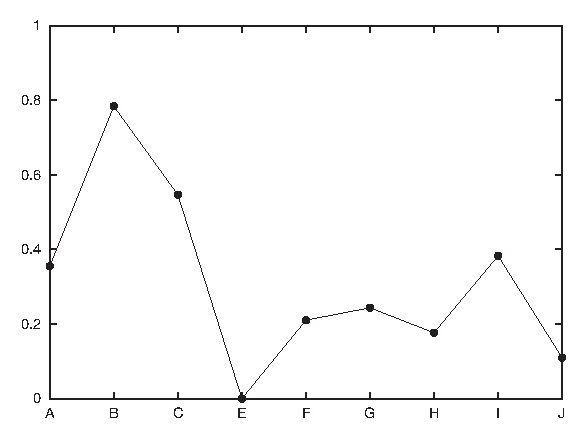
\includegraphics{img/parallel1}}
  \caption{A single record (\ie, a single data point) from a
    multivariate data set shown in a parallel coordinate plot.}
  \label{fig:parallel1}\vspace*{-6pt}
\end{figure}

The main use of parallel coordinate plots is to find clusters in
high-dimensional data sets. For example, in Figure \ref{fig:parallel2},
we can see that the data forms two clusters for the quantity labeled
B: one around $0.8$ and one around $0$. Furthermore, we can see that 
most records for which B is $0$, tend to have higher values of C 
than those that have a B near $0.8$. And so~on.

\begin{figure}
   \centerline{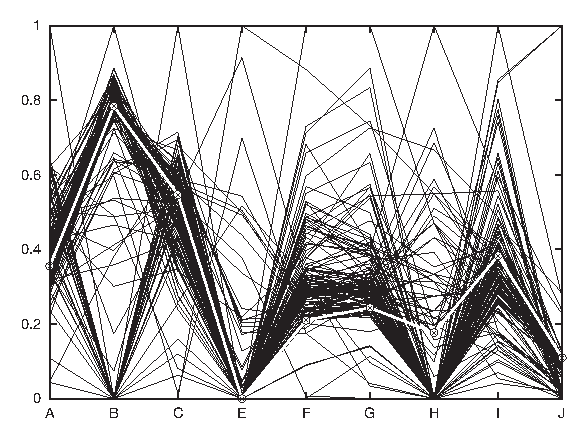
\includegraphics{img/parallel2}}
  \caption{All records from the data set shown in a parallel
    coordinate plot. The record shown in Figure \ref{fig:parallel1} is
    highlighted.}
  \label{fig:parallel2}\vspace*{-6pt}
\end{figure}

A few technical points should be noted about parallel coordinate
plots:

\begin{itemize}
\item You will usually want to rescale the values in each
  coordinate to the unit interval via the linear transformation
  (also see Appendix \ref{app:calculus}):
  % 
  \[
  x_{{\rm scaled}} 
    = \frac{x - x_{{\rm min}}}{x_{{\rm max}} - x_{{\rm min}}}
  \]
  % 
  This is not mandatory, however. There may be situations where
  you care about the absolute positions of the points along the
  coordinate axis or about scaling to a different interval.
\item The appearance of parallel coordinate plots depends strongly on
  the order in which the coordinate lines are drawn: rearranging them
  can hide or reveal structure. Ideally, you have access to a tool
  that lets you reshuffle the coordinate axis interactively.
\item Especially for larger data sets (several hundreds of points
  or more), overplotting of lines becomes a problem. One way to deal
  with this is through ``alpha blending'': lines are shown as
  semi-transparent, and their visual effects are combined where they
  overlap each other.
\item Similarly, it is often highly desirable to be able to select a
  set of lines and highlight them throughout the entire graph---for
  example, to see how data points that are clustered in one dimension
  are distributed in the other dimensions.
\item Instead of combining points on adjacent coordinate axes with
  straight lines that have sharp kinks at the coordinate axes, one
  can use smooth lines that pass the coordinate axes without kinks.
\end{itemize}

All of these issues really are \emph{tool} issues, and in fact
parallel coordinates don't make sense without a tool that supports
them natively and includes good implementations of the features just
described. This implies that parallel coordinate plots serve less as
finished, static graphs than as an interactive tool for exploring a
data set.

Parallel coordinate plots still seem pretty novel. The idea itself has
been around for about 25 years, but even today, tools that support
parallel coordinates plots \emph{well} are far from common place.

What is not yet clear is how useful parallel coordinate plots really
are. On the one hand, the concept seems straightforward and easy
enough to use. On the other hand, I have found the experience of
actually trying to apply them frustrating and not very fruitful. It is
easy to get bogged down in technicalities of the plot (ordering and
scaling of coordinate axes) with little real, concrete insight
resulting in the end. The erratic tool situation of course does not
help.  I wonder whether more computationally intensive methods (\eg,
principal component analysis---see Chapter \ref{ch:reduction}) do not
give a better return on investment overall.  But the jury is still
out.
\index{multivariate analysis!parallel coordinate plots|)}%
\index{parallel coordinate plots|)}%

\vspace*{-6pt}
% ============================================================
\section{Interactive Explorations}

\index{multivariate analysis!interactive explorations|(} 

All the graphs that we have discussed so far (in this and the
preceding chapters) were by nature \emph{static}. We prepared graphs,
so that we then could study them, but this was the extent of our
interaction.  If we wanted to see something different, we had to
prepare a new graph.

In this section, I shall describe some ideas for \emph{interactive}
graphics: graphs that we can change directly in some way without
having to re-create them anew.

Interactive graphics cannot be produced with paper and pencil, not
even in principle: they \emph{require} a computer. Conversely, what we
can do in this area is even more strongly limited by the tools or
programs that are available to us than for other types of graphs. In
this sense, then, this section is more about \emph{possibilities} than
about \emph{realities} because the tool support for interactive
graphical exploration seems (at the time of this writing) rather poor.

\subsection{Querying and Zooming}

\index{querying and zooming, multivariate analysis}
\index{zooming and querying, multivariate analysis} 

Interaction with a graph does not have to be complicated. A very
simple form of interaction consists of the ability to select a point
(or possibly a group of points) and have the tool display additional
information about it. In the simplest case, we hover the mouse pointer
over a data point and see the coordinates (and possibly additional
details) in a tool tip or a separate window. We can refer to this
activity as \emph{querying}.

Another simple form of interaction would allow us to change aspects of
the graph directly using the mouse.  Changing the plot range (\ie,
\emph{zooming}) is probably the most common application, but I could
also imagine to adjust the aspect ratio, the color palette, or
smoothing parameters in this way. (Selecting and highlighting a subset
of points in a parallel coordinate plot, as described earlier, would
be another application.)

Observe that neither of these activities is inherently
``interactive'': they all would also be possible if we used paper and
pencil. The interactive aspect consists of our ability to invoke them
in real time and by using a graphical input device (the mouse).

\vspace*{-9pt}
\subsection{Linking and Brushing}

\index{linking and brushing, multivariate analysis}
\index{brushing and linking, multivariate analysis}
  
The ability to interact directly with graphs becomes much more
interesting once we are dealing with multiple graphs at the same time!
For example, consider a scatter-plot matrix like the one in Figure
\ref{fig:splom}. Now imagine we use the mouse to select and highlight
a group of points in one of the subplots. If the graphs are
\emph{linked}, then the symbols corresponding to the data points
selected in one of the subplots will also be highlighted in all other
subplots as well.

% --- XXX : need a ref to an example here

Usually selecting some points and then highlighting their
corresponding symbols in the linked subgraphs requires two separate
steps (or mouseclicks). A real-time version of the same idea is called
\emph{brushing}: any points currently under the mouse pointer are
selected and highlighted in all of the linked subplots.

Of course, linking and brushing are not limited to scatter-plot
matrices, but they are applicable to any group of graphs that show
different aspects of the same data set.  Suppose we are working with a
set of histograms of a multivariate data set, each histogram showing
only one of the quantities.  Now I could imagine a tool that allows us
to select a bin in \emph{one} of the histograms and then highlights
the contribution from the points in that bin in all the other
histograms.

% --- XXX : need a ref to an example here
\vspace*{-9pt}
\subsection{Grand Tours and Projection Pursuits}

\index{grand tours and projection pursuits, multivariate analysis}
\index{projection pursuits and grand tours, multivariate analysis}
 
Although linking and brushing allow us to interact with the data, they
leave the graph itself static. This changes when we come to
\emph{Grand Tours} and \emph{Projection Pursuits}. Now we are talking
about truly animated graphics!

Grand Tours and Projection Pursuits are attempts to enhance our
understanding of a data set by presenting many closely related\vadjust{\pagebreak}
projections in the form of an animated ``movie.'' The concept is
straightforward: we begin with some projection and then continuously
move the viewpoint around the data set. (For a three-dimensional data
set, you can imagine the viewpoint moving on a sphere that encloses
the data.)

In Grand Tours, the viewpoint is allowed to perform essentially a
random walk around the data set. In Projection Pursuits, the viewpoint
is moved so that it will improve the value of an index that measures
how ``interesting'' a specific projection will appear.  Most indices
currently suggested measure properties such as deviation from Gaussian
behavior. At each step of a Pursuit, the program evaluates several
possible projections and then selects the one that most improves the
chosen index. Eventually, a Pursuit will reach a local maximum for the
index, at which time it needs to be restarted from a different
starting point.

Obviously, Tours and Pursuits require specialized tools that can
perform the required projections---and do so in real time.  They are
also exclusively exploratory techniques and not suitable for
preserving results or presenting them to a general audience.

Although the approach is interesting, I have not found Tours to be
especially useful in practice. It can be confusing to watch a movie of
essentially random patterns and frustrating to interact with
projections when attempting to explore the neighborhood of an
interesting viewpoint.

\vspace*{-9pt}
\subsection{Tools}

\index{multivariate analysis!tools|(}
 
All interactive visualization techniques require suitable tools and
computer programs; they cannot be done using paper-and-pencil methods.
This places considerable weight on the quality of the available tools.
Two issues stand out.

\begin{itemize}
\item It seems difficult to develop tools that support interactive
  features and are sufficiently general at the same time. For example,
  if we expect the plotting program to show additional detail on any
  data point that we select with the mouse, then the input (data) file
  will have to contain this information---possibly as metadata.  But
  now we are talking about relatively complicated data sets, which
  require more complicated, structured file formats that will be
  specific to each tool. So before we can do anything with the data,
  we will have to transform it into the required format. This is a
  significant burden, and it may make these methods infeasible in
  practice.  (Several of the more experimental programs mentioned in
  the Workshop section in this chapter are nearly unusable on actual
  data sets for exactly this reason.)
\item A second problem concerns performance. Brushing, for instance,
  makes sense only if it truly occurs in real time---without any
  discernible delay as the mouse pointer moves. For a large data set
  and a scatter-plot matrix of a dozen attributes, this means updating
  a few thousand points in real time. Although by no means infeasible,
  such responsiveness does require that the tool is written with an
  eye toward performance and using appropriate technologies. (Several
  of the tools mentioned in the Workshop exhibit serious performance
  issues on real-world data sets.)
\end{itemize}

A final concern involves the overall design of the user interface. It
should be easy to learn and easy to use, and it should support the
activities that are actually required. Of course, this concern is not
specific to data visualization tools but common to all programs with
a graphical user interface.
\index{multivariate analysis!interactive explorations|)} 

\vspace*{-9pt}
% ============================================================
\section{Workshop:  Tools for Multivariate Graphics}

Multivariate graphs tend to be complicated and therefore require good
tool support even more strongly than do other forms of graphs.  In
addition, some multivariate graphics are highly specialized (\eg,
mosaic plots) and cannot be easily prepared with a general-\break purpose
plotting tool.

That being said, the tool situation is questionable at best.  Here
are three different starting points for exploration---each with its
own set of difficulties.

\vspace*{-9pt}
\subsection{R}

\index{R statistical analysis package} 
\index{software!R statistical analysis package}

R is not a plotting tool per se; it is a statistical analysis package
and a full development environment as well. However, R has always
included pretty extensive graphing capabilities. R is particularly
strong at ``scientific'' graphs: straightforward but highly accurate
line diagrams.

Because R is not simply a plotting tool, but instead a full data
manipulation and programming environment, its learning curve is rather
steep; you need to know a lot of different things before you can do
anything. But once you are up and running, the large number of
advanced functions that are already built in can make working with R
very productive. For example, the scatter-plot matrix in Figure
\ref{fig:splom} was generated using just these three commands:

\begin{verbatim}
d <- read.delim( "wines", header=T )

pairs(d)

dev.copy2eps( file="splom.eps" )
\end{verbatim}

(the R command \texttt{pairs()} generates a plot of all pairs---\ie, a
scatter-plot matrix). The scatter plot in Figure \ref{fig:coplot1} and
the co-plot in Figure \ref{fig:coplot2} were generated using:

\begin{verbatim}
d <- read.delim( "data", header=F )
names( d ) <- c( "x", "a", "y" )

plot( y ~ x, data=d )
dev.copy2eps( file='coplot1.eps' )

coplot( y ~ x | a, data=d )
dev.copy2eps( file='coplot2.eps' )
\end{verbatim}

Note that these are the \emph{entire} command sequences, which include
reading the data from file and writing the graph back to disk! We'll
have more to say about R in the Workshop sections of Chapters
\ref{ch:statistics} and \ref{ch:reduction}.

R has a strong culture of user-contributed add-on packages. For
multiplots consisting of subplots arranged on a regular grid (in
particular, for generalized co-plots), you should consider the
\texttt{lattice} package, which extends or even replaces the
functionality of the basic R graphic systems. This package is part of
the standard R distribution.

\vspace*{-6pt}
\subsection{Experimental Tools}

If you want to explore some of the more novel graphing ideas, such as
parallel coordinate plots and mosaic plots, or if you want to try out
interactive ideas such as brushing and Grand Tours, then there are
several options open to you. All of them are academic research
projects, and all are highly experimental. (In a way, this is a
reflection of the state of the field: I don't think any of these novel
plot types have been refined to a point where they are clearly
useful.)

\begin{itemize}
\item The ggobi project (\url{http://www.ggobi.org}) allows brushing
  in scatter-plot matrices and parallel coordinate plots and includes
  support for animated tours and pursuits.

\item Mondrian (\url{http://www.rosuda.org/mondrian}) is a Java
  application that can produce mosaic plots (as well as some other
  multivariate graphs).
\end{itemize}

Again, both tools are academic research projects---and it shows. They
are technology demonstrators intended to try out and experiment with
new graph ideas, but neither is anywhere near production strength.
Both are rather fussy about the required data input format, their
graphical user interfaces are clumsy, and neither includes a proper way to
export graphs to file (if you want to save a plot, you have to take a
screenshot). The interactive brushing features in ggobi are slow,
which makes them nearly unusable for realistically sized data sets.
There are some lessons here (besides the intended ones) to be learned
about the design of tools for statistical graphics. (For instance, GUI
widget sets do not seem suitable for interactive visualizations: they
are too slow. You have to use a lower-level graphics library instead.)

Other open source tools you may want to check out are Tulip
(\url{http://tulip.labri.fr}) and ManyEyes
(\url{http://manyeyes.alphaworks.ibm.com/manyeyes}). The latter
project is a web-based tool and community that allows you to upload
your data set and generate plots of it online.

A throwback to a different era is OpenDX
(\url{http://www.research.ibm.com/dx}).  Originally designed by IBM in
1991, it was donated to the open source community in 1999. It
certainly feels overly complicated and dated, but it does include a
selection of features not found elsewhere.

\vspace*{-6pt}
\subsection{Python Chaco Library}

\index{Python Chaco library!} 
\index{software!Python}
 
The Chaco library (\url{http://code.enthought.com/projects/chaco/}) is
a Python library for two-dimensional plotting. In addition\vadjust{\pagebreak} to the
usual line and symbol drawing capabilities, it includes easy support
for color and color manipulation as well as---more importantly---for
real-time user interaction.

Chaco is an exciting toolbox if you plan to experiment with writing
your own programs to visualize data and interact with it. However, be
prepared to do some research: the best available documentation seems
to be the set of demos that ship with it.

Chaco is part of the Enthought Tool Suite, which is developed by
Enthought, Inc., and is available under a BSD-style license.

\index{multivariate analysis!tools|)}

% ============================================================
\section{Further Reading}

\begin{itemize}

\item \cit{Graphics of Large Datasets: Visualizing a Million}{Antony
    Unwin, Martin Theus, and Heike Hofmann}{Springer}{2006} 
  This is a modern book that in many ways describes the state of the
  art in statistical data visualization. Mosaic plots, glyph plots,
  parallel coordinate plots, Grand Tours---all are discussed here.
  Unfortunately, the basics are neglected: standard tools like
  logarithmic plots are never even mentioned, and simple things like
  labels are frequently messed up.  This book is nevertheless
  interesting as a survey of some of the state of the art.

\item \cit{The Elements of Graphing Data}{William S.\ Cleveland}{2nd ed.,
    Hobart Press}{1994} 
  This book provides an interesting counterpoint to the book by Unwin
  and colleagues. Cleveland's graphs often look pedestrian, but he
  thinks more deeply than almost anyone else about ways to incorporate
  more (and more quantitative) information in a graph. What stands out
  in his works is that he explicitly takes human perception into
  account as a guiding principle when developing new graphs. My
  discussion of scatter-plot matrices and co-plots is heavily
  influenced by his careful treatment.

\item \cit{Gnuplot in Action: Understanding Data with Graphs}{Philipp 
    K.\ Janert}{Manning Publications}{2010}
  Chapter 9 of this book contains additional details on and examples
  for the use of color to prepare false-color plots, including
  explicit recipes to create them using gnuplot. But the principles
  are valid more generally, even if you use different tools.

\item 
{\it Why Should Engineers and Scientists Be Worried About
    Color?} {B.\ E.\ Rogowitz and L.\ A.\
    Treinish.} {\url{http://www.research.ibm.com/people/l/lloydt/color/color.HTM}.} {1995.}
  This paper contains important lessons for false-color plots,
  including the distinction between segmentation and smooth variation
  as well as the difference between hue- and luminance-based palettes.
  The examples were prepared using IBM's (now open source) OpenDX
  graphical Data Explorer.

\item \cit{Escaping RGBland: Selecting Colors for Statistical
    Graphics}{A.\ Zeileis, K.\ Hornik, and 
P.~Murrell}{\url{http://statmath.wu.ac.at/}$\sim$\url{zeileis/papers/Zeileis+Hornik+Murrell-2009.pdf}}{2009}
  This is a more recent paper on the use of color in graphics. It
  emphasizes the importance of perception-based color spaces, such as
  the HCL model.
\end{itemize}

\index{data analysis!multivariate analysis|)} 
\index{multivariate analysis|)} 

\clearpage

\thispagestyle{empty}

\cleardoublepage